\chapter{Conclusioni}
\label{cap5}
\setcounter{figure}{0}


\section{Lavoro svolto}
In questa tesi abbiamo cercato, attraverso dati sperimentali, di provare l'esistenza di una correlazione tra username di SNS differenti che connette individui reali tra di loro e di trovare questa correlazione. Per farlo, abbiamo progettato e implementato una soluzione
che consente di stabilire la correlazione di identità tra profili di individui presenti su diversi social networks online. Abbiamo collezionato un campione di $\sim$ 100000 username collegati ad altri username, di servizi differenti, per i quali è nota l'appartenenza allo stesso individuo. Per raccogliere queste informazioni abbiamo individuato una pratica e valida fonte di dati nei servizi di \textit{social network aggregation}, che permettono di collezionare contenuti da diversi \textit{social network services} in una presentazione unificata. Attraverso questi è possibile visualizzare tutte le attività di un utente sui diversi social network che questo ha deciso di far seguire all'aggregatore. In seguito, attraverso una tecnica per l'estrazione di dati da pagine web, conosciuta come \textit{web scraping} o \textit{web data extraction}, è stata recuperata ed elaborata l'informazione di interesse, ovvero un elenco di profili di social network services appartenenti alla stessa persona. Su questi dati abbiamo cercato di individuare una serie di modelli comportamentali mostrati dagli utenti nello scegliere uno username ricercando pattern, che generando ridondanza di informazione, possono essere utili per la funzione di identificazione \textit{f}(\textit{U,c}), così definita

\[ f(U,c) = \left\{
\begin{array}{l l}
	1 & \quad \text{se \textit{c} e l'insieme \textit{U} appartengono a \textit{I} ;}\\
	0 & \quad \text{altrimenti}
	\end{array} \right.\] dove \textit{U} è l'informazione a priori che abbiamo di un individuo \textit{I}, in questo caso un insieme di username, e \textit{c} è lo username candidato di cui vorremmo testare l'appartenenza allo stesso \textit{I}.
Questa funzione di identificazione è stata realizzata attraverso l'implementazione di un modello predittivo, in particolare un modello di riconoscimento di pattern, addestrato a riconoscere i pattern comportamentali descritti precedentemente. Questo modello è capace di attuare predizioni accurate in base alle osservazioni fatte sui dati estratti. In particolare, sono stati testati diversi modelli di apprendimento supervisionato, come Support Vector Machine (SVM) utilizzando dapprima un kernel RBF e in seguito affrontando il problema utilizzando SVM senza kernel, riscontrando performance simili, indicandoci che probabilmente il problema era risolvibile linearmente. Con il crescere del numero delle features e dei samples a disposizione, crescevano anche i tempi di esecuzione dell'algoritmo e la memoria richiesta dal calcolo, diventando troppo onerosi. È nata così la necessità di passare a un modello di classificatori diversi, conosciuti come “online”, che hanno permesso di affrontare il problema con risorse di tempo e memoria molto più limitate. Tra questi abbiamo individuato e testato due algoritmi online: Stochastic Gradient Descent e Passive Aggressive.

\section{Risultati}
Abbiamo testato due algoritmi di classificatori binari online, Stochastic Gradient Descent (SGD) e Passive Aggressive (PA) usando come metriche per misurare la performance del modello di classificazione, l'Accuracy (ACC), la F-measure (F1), e la Area Under Curve (AUC) della funzione Receiver Operating Characteristic (ROC). Stochastic Gradient Descent ha portato a risultati migliori rispetto PA, raggiungendo il 93.53\% di Accuracy, una F1 del 93.22\% e 93.53\% come AUC. Ad ogni modo, SGD risulta essere più sensibile al variare di numero di features rispetto a PA che invece mantiene un'accuratezza quasi costante al variare di queste.\newline Abbiamo infatti testato le performance di entrambi i classificatori variando le classi di features presentate nel capitolo due, variandone quindi il numero e riducendole fino a 10 sulle 358 implementate, ottenendo 91.55\% di Accuracy e il 91.94\% come F1 utilizzando SGD, e il 91.66\% di Accuracy con il 90.84\% come F1 utilizzando Passive Aggressive. Abbiamo inoltre analizzato l'andamento del classificatore filtrando il dataset variando il numero minimo di priors e utilizzando solamente il sottoinsieme di 10 features. Usando un set ristretto di solo 10 features, il classificatore spazia da una accuratezza del 91.5\% utilizzando l'intero dataset fino a una accuratezza del 100\% utilizzando i profili con il massimo numero di priors username (26). Riassumendo, riteniamo Stochastic Gradient Descent l'algoritmo migliore per affrontare il problema di categorizzazione preposto in questa tesi, e individuiamo Passive Aggressive come algoritmo con risultati migliori per un numero ristretto di features.\newline

\section{Sviluppi futuri}

Contemporaneamente al lavoro svolto in questa tesi abbiamo individuato un'altra fonte dalla quale potere estrapolare dati riguardanti username di utenti su diversi social network. Trattasi della piattaforma per l'apprendimento di lingue \textbf{Duolingo}\footnote{https://www.duolingo.com/}, mediante lezioni e test presentate con un modello di gamification. Il dataset ottenuto consiste in una collezione più ricca, con maggior numero di profili, e più omogenea, con un minore numero di social networks presenti. Il servizio permette ai proprio utenti di accedere utilizzando il proprio profilo Twitter, Facebook o Google+, ed è possibile visualizzare quali sono i profili associati. Nel migliore dei casi avremo quindi almeno una associazione di username tra due servizi diversi: quello selezionato per Duolingo, sempre presente, e quello del SNS utilizzato per l'accesso. La collezione è stata estratta effettuando il crawling attraverso le relazioni di following e follower presenti sul servizio, utilizzando una strategia BFS\footnote{Breadth-first search} e il mio profilo personale\footnote{https://www.duolingo.com/mattiamattia} come nodo di partenza, impostando un limite di profondità di ricerca a 6. Visitando nodi del grafo casualmente, e non partendo dal mio profilo, avrei probabilmente ottenuto un dataset con meno bias, ma ero interessato anche ad analizzare la mia ego-network di Duolingo. Comunque, avendo impostato un limite di profondità abbastanza alto, il numero di profili ricavato è sufficientemente alto per garantire una certa uniformità nei dati ricavati. Sono stati estratti $\sim$600000 profili, di cui di 350000 hanno utilizzato Facebook, 50000 hanno utilizzato Google+ e 7000 Twitter\footnote{Le cifre sono arrotondate}. Inoltre, alcuni utenti hanno collegato più SNS, ad esempio di circa $\sim$21000 utenti conosciamo sia il profilo Facebook che Google+ e, ovviamente, Duolingo. Con la tecnica mostrata in 3.1.2 è possibile espandere ulteriormente il numero di coppie di username. In Fig1 riportiamo un sottoinsieme della ego-network ricavata (bolla 4), dove i colori dei nodi rappresentano la lingua di apprendimento con punteggio più alto, e la grandezza è indice sia del numero di connessioni sia del punteggio raggiunto. Una versione interattiva del grafo, filtrabile per lingua di apprendimento e indegree e con la possibilità di animare la disposizione dei nodi\footnote{Secondo l'algoritmo Force Atlas II} è raggiungibile a http://mattiadmr.com/graph/duolingo/filter.html\footnote{Web app realizzata in HTML e Javascript}\footnote{Per la rappresentazione del grafo usiamo la libreria Sigma.js}

\begin{figure}[bp!]
	\centering
	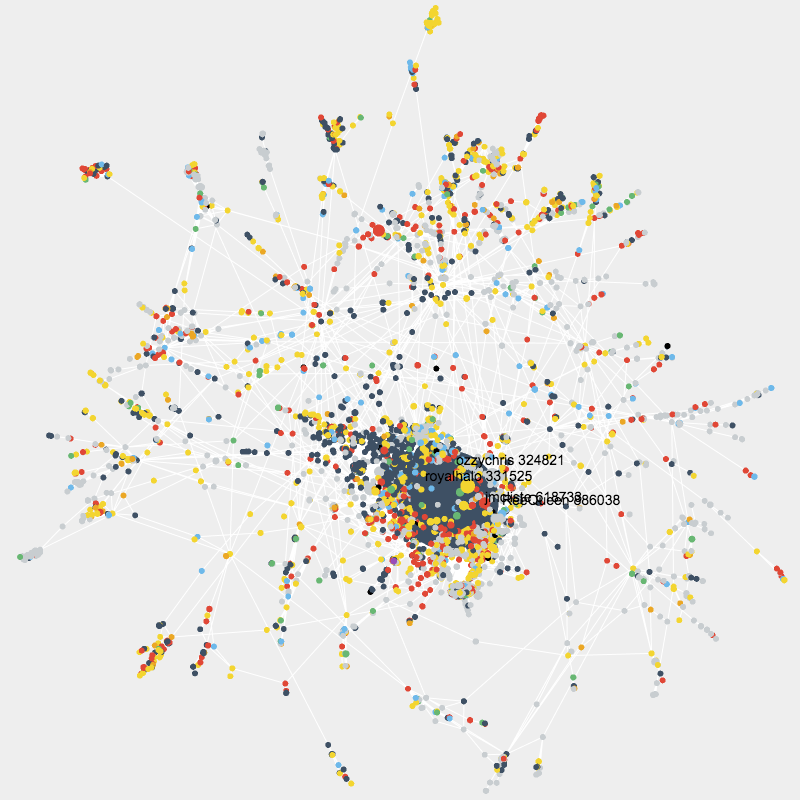
\includegraphics[width=110mm]{chapters/img/duograph.png}
	\caption{Ego-network di Duolingo, utilizzando il mio profilo personale come nodo di partenza. \label{overflow}}
\end{figure}
